\subsection{Multi-Sensor Simulation Campaign for Method Development}
\label{sec:multisensor-benchmark}

To complement the strategic (MSLA) and tactical (HTLV/DAIDALUS) analyses, we conducted a synchronized multi-modal simulation campaign in Cosys-AirSim to quantify frame-level detectability under identical encounter conditions. For air traffic authorities and ATC-oriented stakeholders, this section is intended as a method-development evidence package: it helps clarify applicability, practical constraints, and integration trade-offs for non-cooperative intruder detection in ABDAA-style concepts. The results are therefore indicative and exploratory, not definitive operational performance claims.

This revision aligns narrative and quantitative RGB elements with \textbf{Experiment~30} (30 encounter scenarios in \texttt{scenarios.py}, \texttt{tools/experiment\_controller.py} with \texttt{--multicam}), as documented in the Point~D technical report structure (Sec.~2.3, \emph{Multi-Sensor Simulation Campaign}). Cross-modal LiDAR/radar summaries retain the methodology and interpretation used there: strict $(\mathrm{run},\mathrm{frame})$ alignment, distance reference from \texttt{telemetry.csv}, and explicit caveats on radar return-presence baselines.

\subsubsection{Objective and evaluation questions}
The campaign addresses three method-oriented operational questions:
\begin{enumerate}
  \item Which sensor tends to detect first under identical run/frame conditions?
  \item How does detection probability vary with intruder distance?
  \item What is the trade-off between detection availability and range consistency?
\end{enumerate}
These questions are used to structure future validation phases and higher-fidelity UTM-oriented evaluations, rather than to claim readiness for direct operational deployment.

\subsubsection{Experimental setup and reproducibility}
\begin{itemize}
  \item \textbf{Simulation environment}: Cosys-AirSim multirotor stack used as a technical campaign platform (not an asserted final operational solution).
  \item \textbf{Controller}: \texttt{tools/experiment\_controller.py} with synchronized capture; Experiment~30 uses \texttt{--rotate-observer}, vertical separation, and optional full sensor suite (RGB, depth, segmentation, IR, dual LiDAR, radar per project settings).
  \item \textbf{RGB / segmentation source layout}: \texttt{dataset\_exp30\_multicam/} with one folder per forward-facing camera---\texttt{front\_center}, \texttt{front\_medium}, \texttt{front\_narrow\_hd}, \texttt{front\_lowcost\_640}---each containing \texttt{run\_*} trees with \texttt{rgb/}, \texttt{seg/}, \texttt{telemetry.csv}.
  \item \textbf{YOLO ground truth}: hull-colour segmentation masks projected to axis-aligned boxes via \texttt{tools/generate\_yolo\_labels.py} (hull BGR \texttt{159\,223\,95}, consistent with the Block casco reference in \texttt{tools/run\_block\_dataset.py}). Outputs per campaign:
  \begin{itemize}
    \item Pooled multicam: \texttt{dataset\_exp30\_multicam\_yolo/} (680 train / 170 val labeled frames).
    \item Per-camera splits: \texttt{dataset\_exp30\_yolo\_lowcost640/}, \texttt{dataset\_exp30\_yolo\_medium/}, \texttt{dataset\_exp30\_yolo\_narrow\_hd/}; \texttt{dataset\_exp30\_frontcenter\_yolo/} (154 train / 39 val) is available for a dedicated \texttt{front\_center} model not yet tabulated below.
  \end{itemize}
  \item \textbf{RGB detector training}: YOLOv8s, ImageNet-pretrained, 100 epochs (default Ultralytics settings with patience~20), AMP on GPU; training size 960 for HD/medium/multicam streams and 640 for the low-cost stream. Weights and curves: \texttt{runs/detect/runs/train/exp30\_*}.
  \item \textbf{Cross-sensor distance reference}: \texttt{dist\_xy\_m} in \texttt{telemetry.csv}. For strict cross-modal tables (below), the Point~D refresh uses a 640-frame synchronized subset and \texttt{front\_narrow\_hd} as primary RGB stream in \texttt{tools/compare\_sensors.py} when detection CSVs are exported to \texttt{runs/detect/}.
  \item \textbf{Sensors in the full benchmark}: RGB + YOLOv8, LiDAR OS128, LiDAR VLP16, Echo Radar (CSM profile / return-presence cueing).
\end{itemize}

Full simulator layout per run (when exporting all modalities):
\begin{center}
\texttt{rgb/ seg/ depth/ lidar\_os128/ lidar\_vlp16/ radar/ telemetry.csv}
\end{center}

\paragraph{Implementation artifacts}
\begin{itemize}
  \item RGB training/inference: \texttt{tools/generate\_yolo\_labels.py}, \texttt{tools/train\_yolo.py}, \texttt{tools/detect\_rgb.py}, \texttt{tools/detect\_rgb\_cameras.py}.
  \item Report figures (metrics bars, mAP curves, dataset sizes, distance-band chart): \texttt{tools/build\_multisensor\_report\_figures.py} $\rightarrow$ \texttt{figures/}.
  \item LiDAR detection: \texttt{tools/detect\_lidar.py}.
  \item Radar detection: \texttt{tools/detect\_radar.py}.
  \item Cross-sensor aggregation: \texttt{tools/compare\_sensors.py}.
  \item Visualization helper: \texttt{tools/vis\_sensors.py}.
\end{itemize}

\begin{figure}[ht]
  \centering
  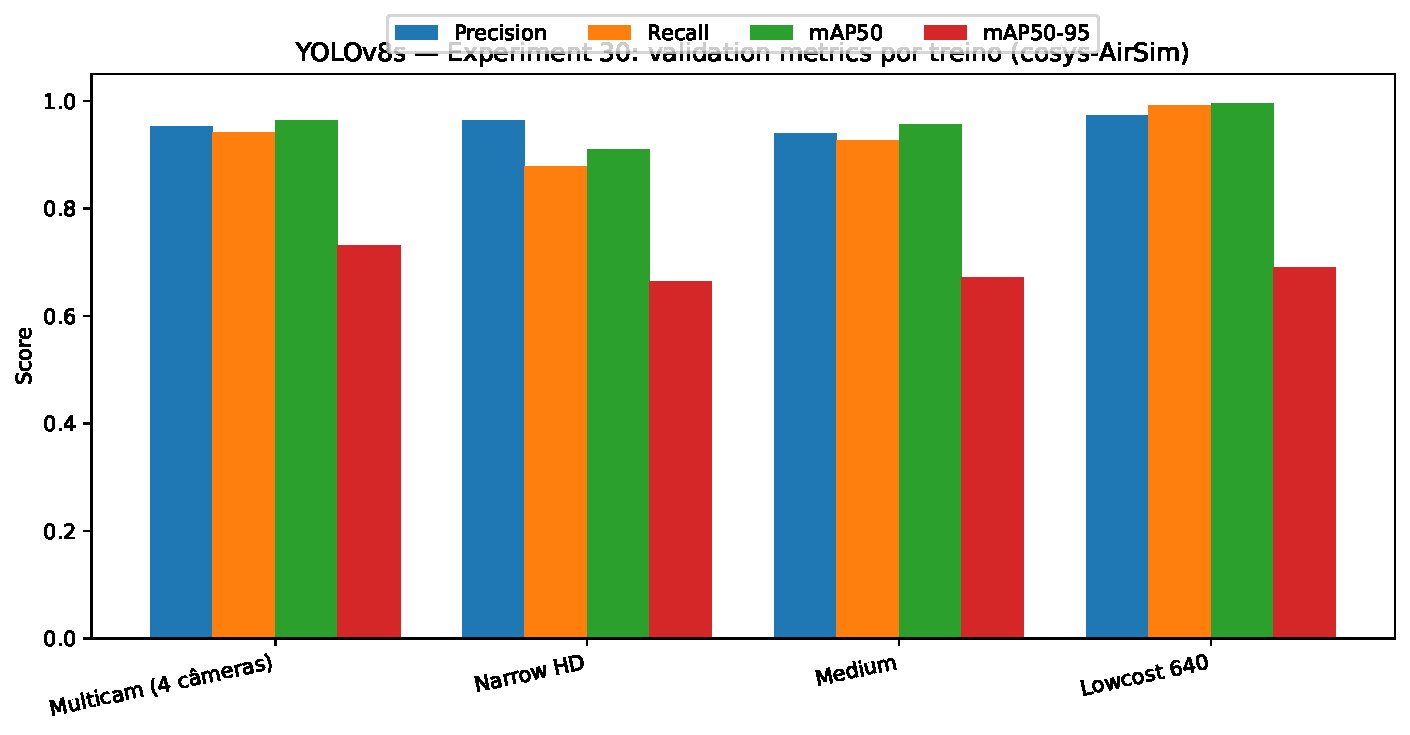
\includegraphics[width=0.92\linewidth]{figures/exp30_yolo_camera_metrics.pdf}
  \caption{Experiment~30: validation precision, recall, mAP50, and mAP50--95 after independent YOLOv8s training per camera stream (and pooled multicam). Low-cost training plateaued at epoch~94 (early stopping).}
  \label{fig:exp30-yolo-metrics}
\end{figure}

\begin{figure}[ht]
  \centering
  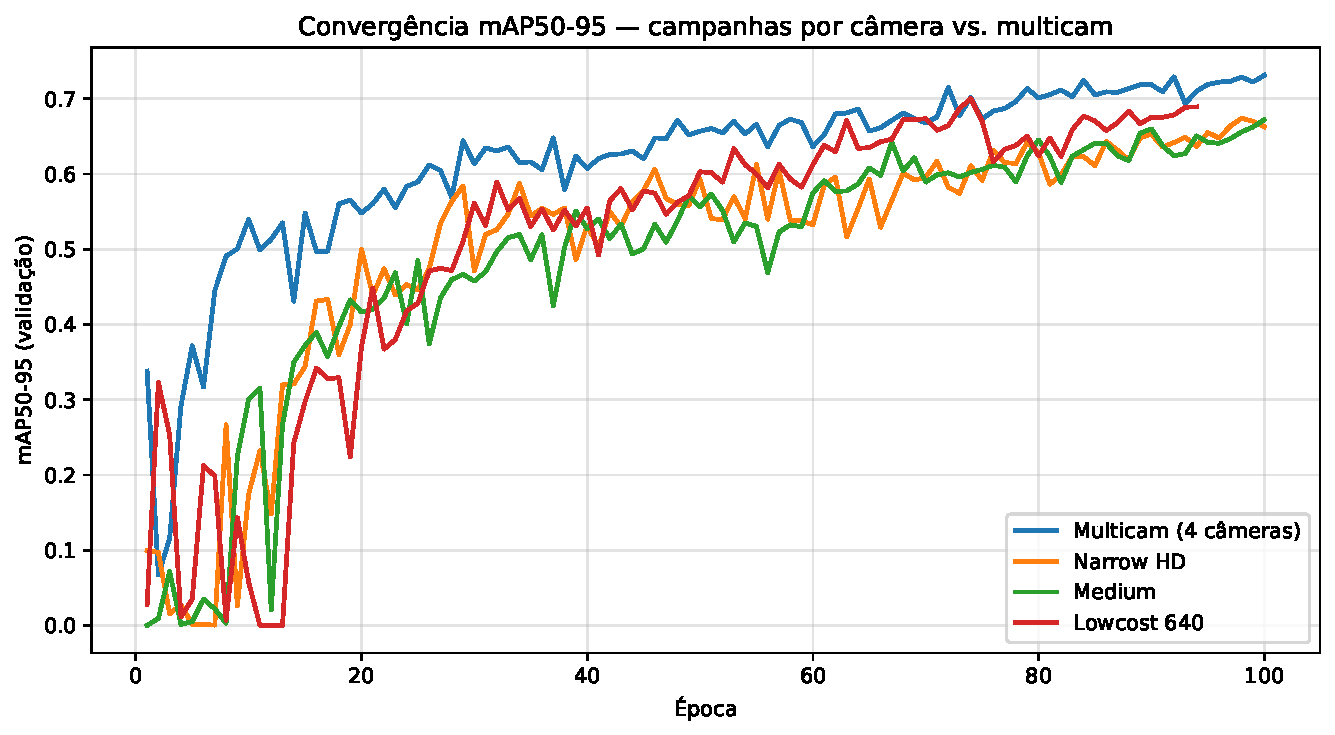
\includegraphics[width=0.92\linewidth]{figures/exp30_yolo_map_curves.pdf}
  \caption{Validation mAP50--95 vs.\ epoch: pooled multicam vs.\ single-sensor datasets. Multicam pooling stabilizes upper-90s mAP50 with the largest validation set (170 images).}
  \label{fig:exp30-yolo-curves}
\end{figure}

\begin{figure}[ht]
  \centering
  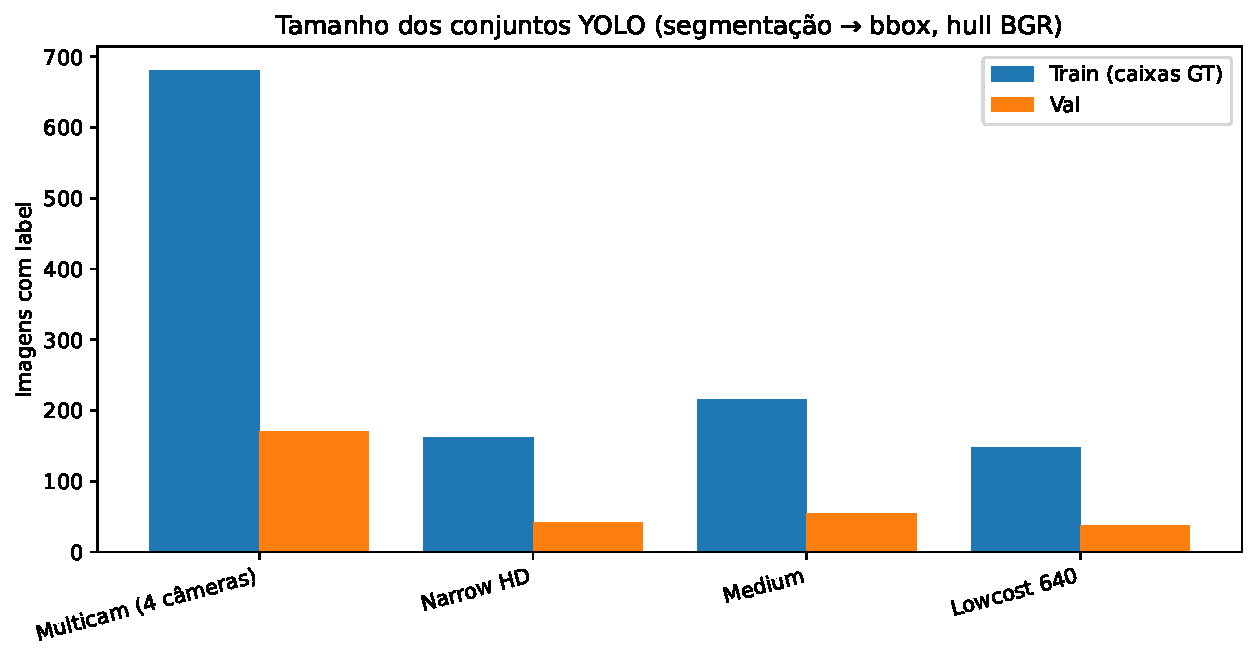
\includegraphics[width=0.85\linewidth]{figures/exp30_yolo_dataset_sizes.pdf}
  \caption{Effective YOLO sample counts after segmentation filtering: the 640\,px stream yields fewer valid hull pixels (many frames skipped); HD/medium streams contribute more labeled frames per scenario.}
  \label{fig:exp30-yolo-sizes}
\end{figure}

\subsubsection{RGB multi-camera evaluation (trained YOLOv8s, Experiment~30)}
\label{sec:rgb-multicam}
Table~\ref{tab:rgb-yolov8s-exp30} summarizes \emph{per-camera training}: each row is a detector trained only on images from that sensor package, evaluated on its held-out split. Table~\ref{tab:rgb-crossval-multicam} reports the \textbf{single multicam-trained} checkpoint (\texttt{best.pt} from \texttt{exp30\_multicam\_yolov8s}) evaluated on each dataset: this tests whether one fused-domain model matches specialist models without retraining.

\begin{table}[ht]
  \centering
  \caption{YOLOv8s on Experiment~30: independent training per camera (validation split). Epochs: 100 (94 for low-cost).}
  \label{tab:rgb-yolov8s-exp30}
  \begin{tabular}{lrrrrrr}
    \hline
    \textbf{Stream} & \textbf{Train} & \textbf{Val} & \textbf{P} & \textbf{R} & \textbf{mAP50} & \textbf{mAP50--95} \\
    \hline
    Pooled multicam & 680 & 170 & 0.952 & 0.941 & 0.964 & 0.731 \\
    \texttt{front\_narrow\_hd} & 162 & 41 & 0.963 & 0.878 & 0.909 & 0.663 \\
    \texttt{front\_medium} & 215 & 54 & 0.939 & 0.926 & 0.956 & 0.672 \\
    \texttt{front\_lowcost\_640} & 148 & 37 & 0.973 & 0.992 & 0.994 & 0.689 \\
    \hline
  \end{tabular}
\end{table}

\begin{table}[ht]
  \centering
  \caption{Cross-evaluation: multicam \texttt{best.pt} on each YAML (same metrics as Ultralytics \texttt{val}). Useful for deployment when only one model is carried.}
  \label{tab:rgb-crossval-multicam}
  \begin{tabular}{lrrrrr}
    \hline
    \textbf{Validation set} & \textbf{Val imgs} & \textbf{P} & \textbf{R} & \textbf{mAP50} & \textbf{mAP50--95} \\
    \hline
    Pooled multicam & 170 & 0.964 & 0.953 & 0.972 & 0.734 \\
    Narrow HD only & 41 & 0.973 & 0.866 & 0.917 & 0.700 \\
    Medium only & 54 & 0.928 & 0.961 & 0.967 & 0.707 \\
    Low-cost only & 37 & 0.991 & 1.000 & 0.995 & 0.741 \\
    \hline
  \end{tabular}
\end{table}

\noindent\textbf{Interpretation.} Specialist low-cost and medium trains achieve very high scores on small validation draws; interpret alongside Fig.~\ref{fig:exp30-yolo-sizes}. The multicam model matches or exceeds single-stream mAP50--95 when evaluated on those splits, supporting a \emph{single checkpoint} for fused simulation data. Narrow HD specialist retains a recall edge on its own split (0.878 vs.\ 0.866 multicam), which may matter for long-range encounters where the narrow FOV crops the intruder.

A dedicated \texttt{front\_center} row is omitted until \texttt{dataset\_exp30\_frontcenter\_yolo} is trained with the same schedule; the pooled multicam set already includes \texttt{front\_center} imagery mixed with the other three streams.

\begin{figure}[ht]
  \centering
  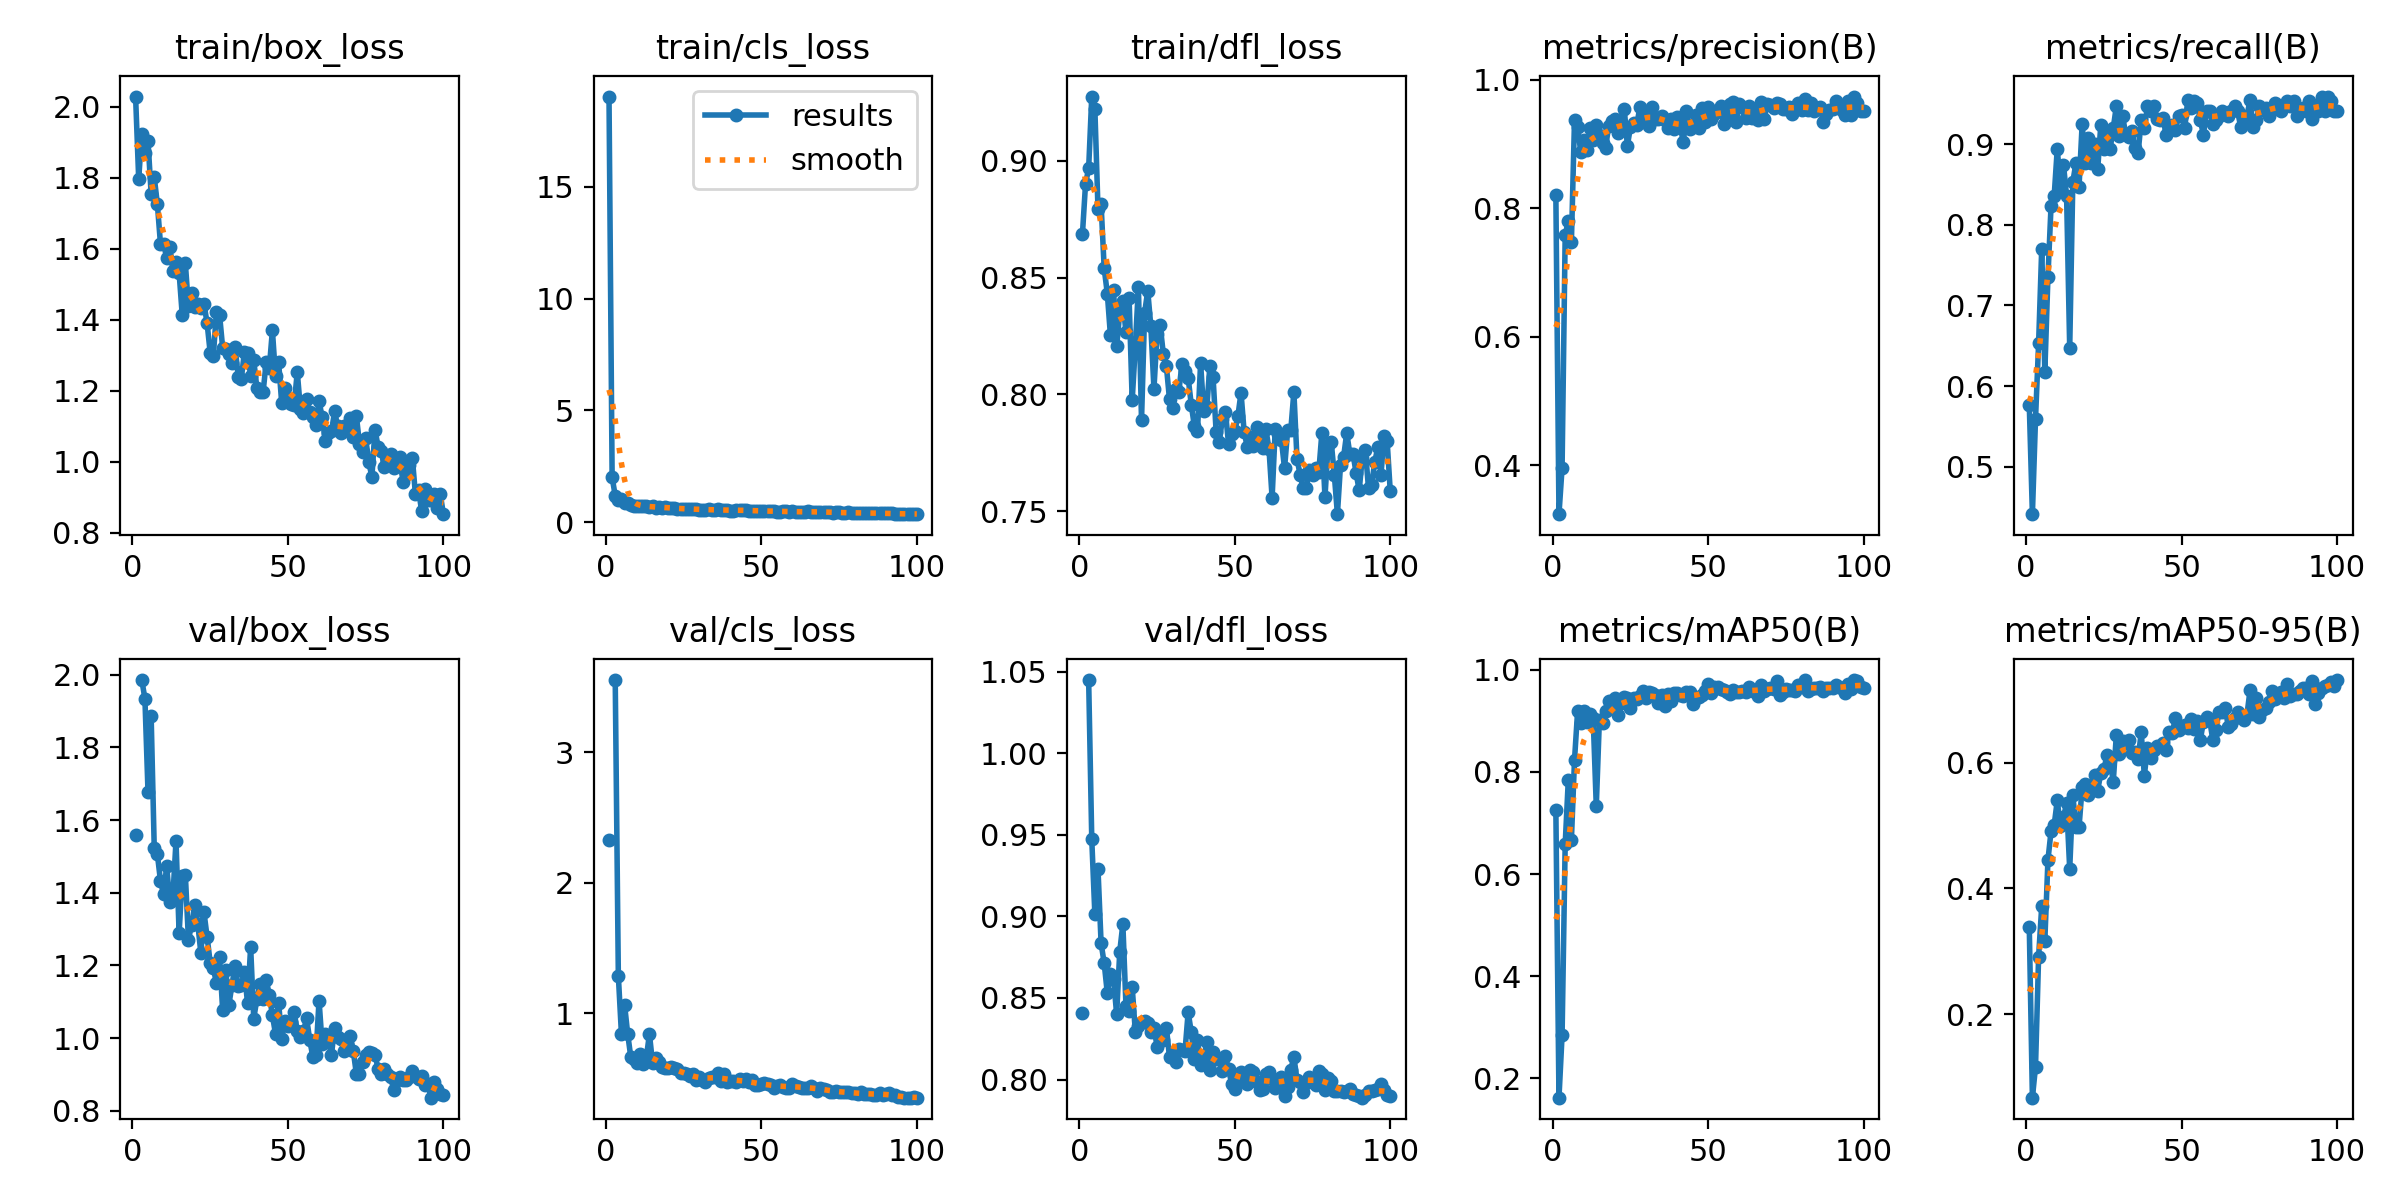
\includegraphics[width=0.75\linewidth]{figures/exp30_multicam_training_results.png}
  \caption{Ultralytics training dashboard for pooled multicam YOLOv8s (loss and validation mAP traces).}
  \label{fig:exp30-multicam-ultra}
\end{figure}

\begin{figure}[ht]
  \centering
  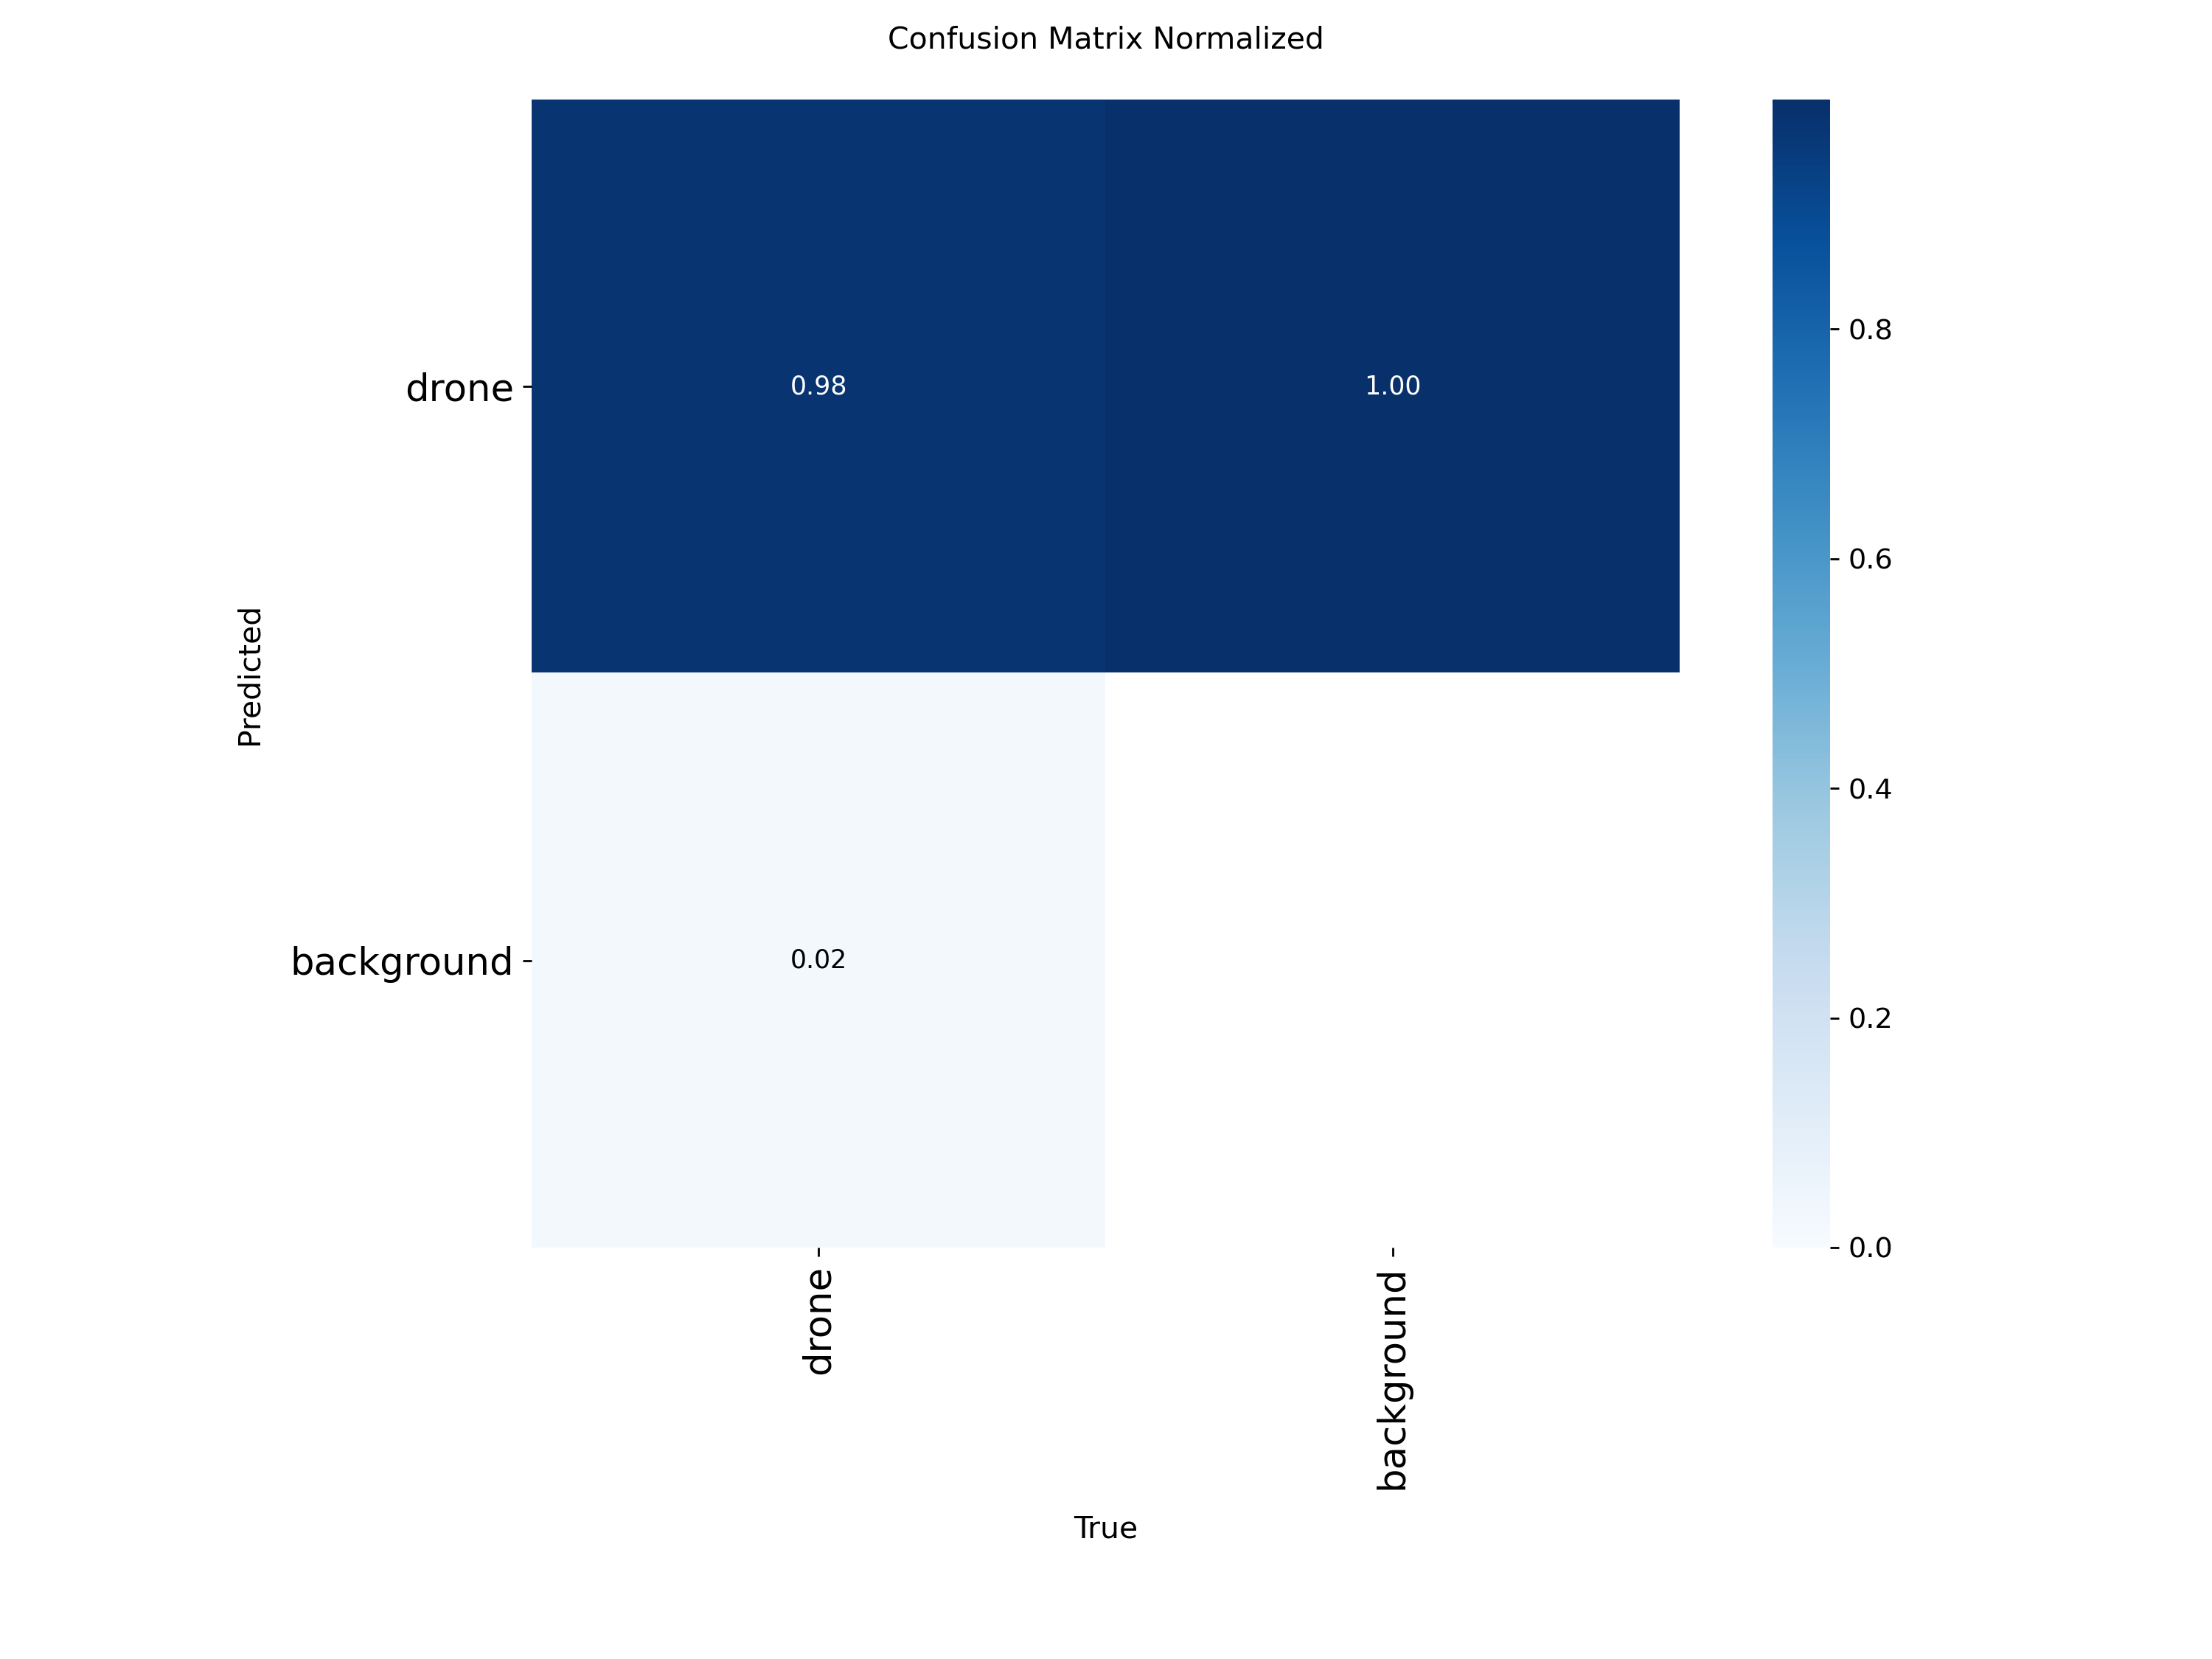
\includegraphics[width=0.62\linewidth]{figures/exp30_multicam_confusion_matrix_normalized.png}
  \caption{Normalized confusion matrix on the multicam validation split (single-class ``drone''; off-diagonal mass reflects score-threshold behaviour at the operating point).}
  \label{fig:exp30-multicam-conf}
\end{figure}

\subsubsection{Cross-sensor detection by distance band (reference benchmark)}
Figure~\ref{fig:exp30-sensor-bands} visualizes the same distance-stratified pattern summarized in Point~D (Tab.~2.3.4): LiDAR OS128 maintains mid-to-high detection rates in tactical bands; VLP16 is sparser; radar remains at 100\% under the return-presence definition; RGB (\texttt{front\_narrow\_hd}, legacy scoring pipeline from the report refresh) stays comparatively low---emphasizing complementarity rather than substitutability.

\begin{figure}[ht]
  \centering
  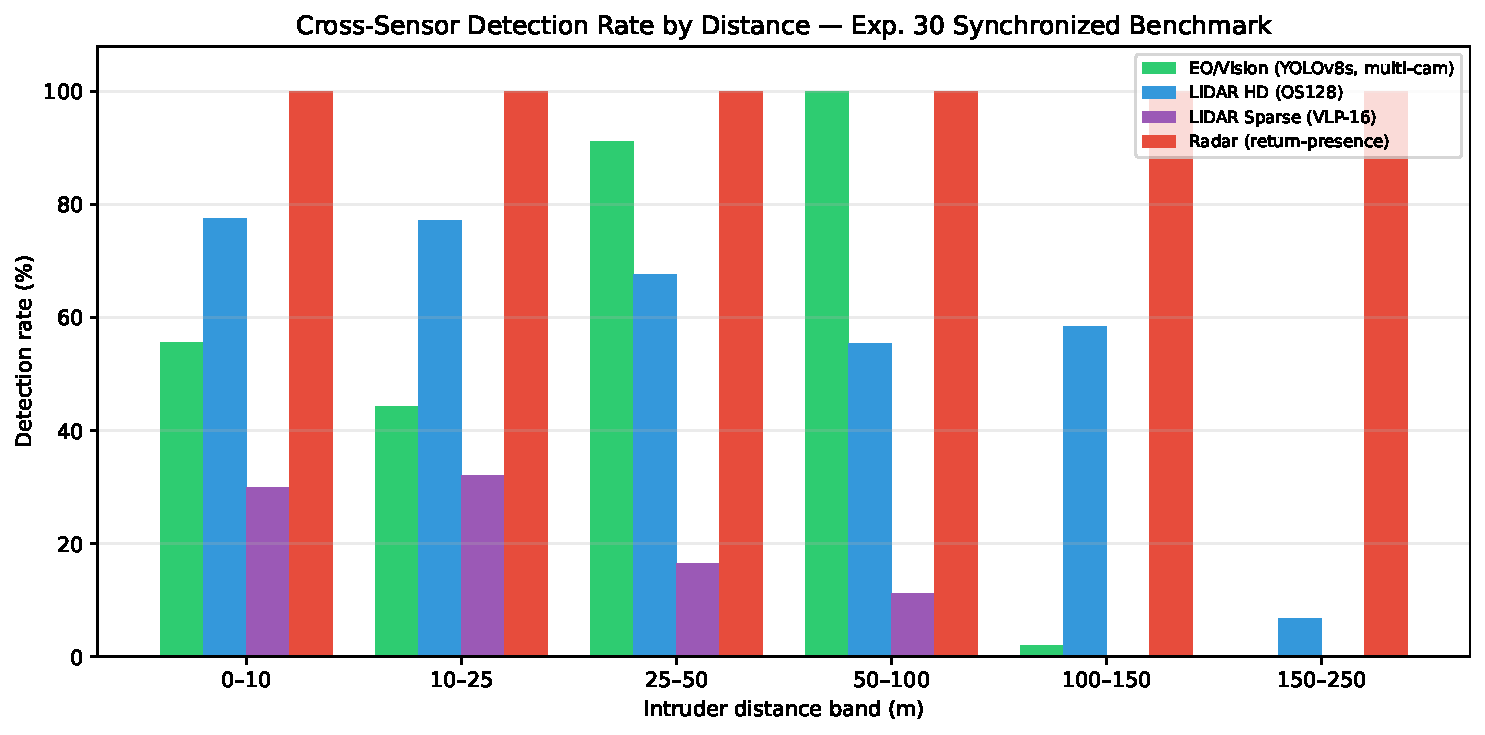
\includegraphics[width=0.95\linewidth]{figures/exp30_sensor_detection_by_distance.pdf}
  \caption{Detection rate (\%) vs.\ ground-truth distance band --- methodology-aligned 640-frame benchmark (RGB column uses HD-primary scoring as in \texttt{compare\_sensors.py}).}
  \label{fig:exp30-sensor-bands}
\end{figure}

\begin{table}[ht]
  \centering
  \caption{Detection rate (\%) by distance band --- refreshed aligned benchmark (640 frames, 29 runs), tabulated form as in Point~D.}
  \label{tab:det-rate-distance}
  \begin{tabular}{lcccc}
    \hline
    \textbf{Distance band (m)} & \textbf{RGB YOLO} & \textbf{LiDAR OS128} & \textbf{LiDAR VLP16} & \textbf{Radar Echo} \\
    \hline
    0--10   &  7.5 & 77.6 & 29.9 & 100.0 \\
    10--25  &  2.8 & 77.1 & 32.1 & 100.0 \\
    25--50  & 10.2 & 67.7 & 16.5 & 100.0 \\
    50--100 &  6.7 & 55.4 & 11.2 & 100.0 \\
    100--150&  1.2 & 58.5 &  0.0 & 100.0 \\
    150--250&  0.0 &  6.7 &  0.0 & 100.0 \\
    \hline
  \end{tabular}
\end{table}

Global frame-level detection rates on the same 640-frame synchronized subset:
\begin{itemize}
  \item RGB YOLO (\texttt{front\_narrow\_hd} aligned stream): 6.1\% (39/640)
  \item LiDAR OS128: 63.1\% (404/640)
  \item LiDAR VLP16: 16.1\% (103/640)
  \item Radar Echo: 100.0\% (640/640)
\end{itemize}

\paragraph{Important interpretation note}
The radar result above corresponds to a \emph{return-presence} detector (valid return in frame), i.e., a high-availability cueing signal. It should not be interpreted as target-class certainty on its own. In this baseline stage, radar prioritizes recall and early warning support, while confirmation and refinement are expected from fusion with LiDAR/vision and SUM/VISA logic.
More broadly, none of the rates in this section should be interpreted as certification-grade thresholds or direct field-equivalent performance; they are campaign outcomes to support model refinement, sensing strategy selection, and next-step test design.

\subsubsection{Condition-level performance (day/dawn/dusk/night)}
Table~\ref{tab:det-rate-light} reports the refreshed 640-frame synchronized benchmark segmented by lighting condition (run-name tags), as in Point~D Sec.~2.3.4.

\begin{table}[ht]
  \centering
  \caption{Detection rate (\%) by lighting condition (640-frame refreshed synchronized benchmark).}
  \label{tab:det-rate-light}
  \begin{tabular}{lccccc}
    \hline
    \textbf{Condition} & \textbf{Frames} & \textbf{RGB} & \textbf{OS128} & \textbf{VLP16} & \textbf{Radar} \\
    \hline
    Day   & 468 & 6.6 & 62.0 & 15.6 & 100.0 \\
    Dawn  &  55 & 0.0 & 58.2 & 14.5 & 100.0 \\
    Dusk  &  54 & 7.4 & 75.9 & 18.5 & 100.0 \\
    Night &  63 & 4.8 & 65.1 & 19.0 & 100.0 \\
    \hline
  \end{tabular}
\end{table}

\subsubsection{Earliest detection and warning relevance}
First-detection winner per run on the refreshed synchronized export (29 runs):
\begin{itemize}
  \item Radar first: 19.1/29 (tie-shared counting)
  \item OS128 first: 9.1/29 (tie-shared counting)
  \item RGB first: 0.6/29 (tie-shared counting)
  \item VLP16 first: 0.2/29 (tie-shared counting)
\end{itemize}

Mean distance at first-detection win:
\begin{itemize}
  \item Radar: mean 116.9\,m, median 117.1\,m (n=29)
  \item OS128: mean 113.2\,m, median 117.1\,m (n=19)
  \item RGB: mean 72.8\,m, median 72.8\,m (n=2)
  \item VLP16: mean 24.6\,m, median 24.6\,m (n=1)
\end{itemize}

These results indicate that radar and high-density LiDAR tend to provide earlier tactical cueing in the evaluated encounter family, while RGB contributes stronger semantic information mainly in favorable close-/mid-range visual conditions. Experiment~30 YOLO training does not change that ordering for the \emph{frame-scoring} baseline in Table~\ref{tab:det-rate-distance}; it \emph{does} improve within-domain RGB bounding-box quality for fused simulation labels (Tables~\ref{tab:rgb-yolov8s-exp30}--\ref{tab:rgb-crossval-multicam}).

\subsubsection{Suggested improvements to the wider Point~D report (narrative and evidence)}
\label{sec:report-improvements}
The following items tighten traceability between simulation, learning, and authority-facing claims without expanding scope beyond method development:
\begin{enumerate}
  \item \textbf{Link Sec.~2.3 to concrete git artefacts}: cite repository paths for Experiment~30 (\texttt{dataset\_exp30\_multicam}, \texttt{runs/detect/runs/train/exp30\_*}, \texttt{figures/exp30\_*}) so reviewers can replay training and export PDFs.
  \item \textbf{Separate ``inference on operational timeline'' from ``mAP on labeled subsets''}: keep Table~\ref{tab:det-rate-distance} (frame hit-rate under legacy detector settings) distinct from Table~\ref{tab:rgb-yolov8s-exp30} (mAP with simulation GT). Add one paragraph stating that replacing the RGB column with the new \texttt{best.pt} requires re-running \texttt{detect\_rgb\_cameras.py} + \texttt{compare\_sensors.py}.
  \item \textbf{Add false-alert and clutter campaign}: Point~D Appendix already flags no-intruder quantification---prioritize it in the executive summary when claiming radar/LiDAR availability.
  \item \textbf{Fusion visuals}: replace static pipeline placeholder with a diagram showing SUM/VISA data flow and where trained YOLO vs.\ heuristic LiDAR enter (Fig.~\ref{fig:multisensor-pipeline} stub below retained until vector artwork is ready).
  \item \textbf{Human-factors}: cross-reference HITL Sec.~2.4.6 with any future alert-rate estimates from nuisance-alert analysis once detector operating thresholds are frozen.
\end{enumerate}

\begin{figure}[ht]
  \centering
  \fbox{\parbox{0.9\linewidth}{\centering \textit{Vector placeholder}: end-to-end pipeline (scenario $\rightarrow$ synchronized capture $\rightarrow$ per-sensor detection $\rightarrow$ fusion / DAIDALUS). Replace with \texttt{figures/pipeline\_multisensor.pdf} when available.}}
  \caption{Multi-sensor experimental pipeline used in the benchmark.}
  \label{fig:multisensor-pipeline}
\end{figure}

\subsubsection{What worked and current limitations}
\paragraph{What worked}
\begin{itemize}
  \item Synchronized multi-modal acquisition and replayable evaluation.
  \item Reproducible per-sensor and cross-sensor scripts; automated LaTeX-oriented figure export for RGB evidence.
  \item Multicam YOLO training generalizes across per-camera validation YAMLs without retraining (Table~\ref{tab:rgb-crossval-multicam}).
\end{itemize}

\paragraph{Current limitations}
\begin{enumerate}
  \item Radar detector is baseline-level (return presence), not class-discriminative.
  \item LiDAR detector is heuristic clustering, not yet trained/class-aware against clutter.
  \item RGB labels derive from ideal simulation segmentation; real-domain gap and weather-domain shift remain open.
  \item Encounter family is mostly frontal/near-frontal; broader angular and occlusion coverage is still needed.
  \item Results are not intended as final operational acceptance evidence; additional high-fidelity and mixed-reality/field-linked validation is required for authority-facing assurance.
\end{enumerate}

\subsubsection{Implication for ABDAA}
The refreshed campaign supports the hybrid ABDAA rationale as a development and evaluation pathway:
\begin{itemize}
  \item Radar for high-availability early cueing and continuity;
  \item OS128 LiDAR for stronger geometric observability in tactical distances;
  \item RGB for semantic confirmation and visual interpretability (with simulation-trained YOLO now documented quantitatively per stream);
  \item SUM/VISA + DAIDALUS to absorb uncertainty and maintain stable, actionable RWC guidance.
\end{itemize}
For authorities and ATC-focused readers, the practical value is not a final ranking of sensors, but a transparent basis to prioritize future UTM evaluation campaigns with broader scenarios, stronger fidelity controls, and progressively stricter validation criteria.

\subsection*{Appendix A --- Technical framework used in the benchmark}
\addcontentsline{toc}{subsection}{Appendix A --- Technical framework used in the benchmark}
\label{app:technical-framework}

\paragraph{A.1 Data contracts}
The technical details in Appendix A document reproducibility-critical tooling and data contracts; they should be read as implementation support for experimentation, not as endorsement of a single final platform architecture.
\begin{itemize}
  \item \textbf{Telemetry}: frame-indexed reference state, including \texttt{dist\_xy\_m}.
  \item \textbf{RGB CSV}: \texttt{camera, split, run, frame, detected, tp, iou, confidence, has\_gt\_label, gt\_distance\_m} (multi-camera export) or legacy single-stream columns via \texttt{detect\_rgb.py}.
  \item \textbf{LiDAR CSV}: \texttt{run, frame, detected, est\_range\_m, n\_points, gt\_distance\_m, range\_error\_m}.
  \item \textbf{Radar CSV}: \texttt{run, frame, detected, est\_range\_m, n\_returns, gt\_distance\_m, range\_error\_m}.
\end{itemize}

\paragraph{A.2 Algorithmic baseline choices}
\begin{itemize}
  \item \textbf{RGB}: YOLOv8 object detection trained on simulation-derived labels (Experiment~30: YOLOv8s, pooled and per-camera).
  \item \textbf{LiDAR}: DBSCAN clustering after zero/near-body filtering.
  \item \textbf{Radar}: valid-return gating and nearest-return range proxy.
  \item \textbf{Comparison}: strict key matching by (\texttt{run}, \texttt{frame}) for same-condition evaluation.
\end{itemize}

\paragraph{A.3 Reproducibility procedure}
\begin{enumerate}
  \item Generate synchronized runs with all sensors enabled (\texttt{tools/run\_experiment30\_dataset.py --multicam --only-post} after capture).
  \item Train / evaluate RGB:
  \begin{itemize}
    \item \texttt{python tools/train\_yolo.py --data dataset\_exp30\_multicam\_yolo/dataset.yaml --model yolov8s.pt --device 0}
    \item \texttt{python tools/build\_multisensor\_report\_figures.py --device 0}
  \end{itemize}
  \item Production inference sweep:
  \begin{itemize}
    \item \texttt{python tools/detect\_rgb\_cameras.py --data-root \ldots{} --model runs/detect/runs/train/exp30\_multicam\_yolov8s/weights/best.pt}
    \item (optional single stream) \texttt{python tools/detect\_rgb.py ...}
    \item \texttt{python tools/detect\_lidar.py --sensor os128}
    \item \texttt{python tools/detect\_lidar.py --sensor vlp16}
    \item \texttt{python tools/detect\_radar.py}
    \item \texttt{python tools/compare\_sensors.py [--primary-rgb-camera front\_narrow\_hd]}
  \end{itemize}
  \item Export representative figures from \texttt{tools/vis\_sensors.py} and \texttt{figures/exp30\_*.pdf}.
\end{enumerate}

\paragraph{A.4 Recommended next-step hardening}
\begin{itemize}
  \item No-intruder clutter campaign for false-alert quantification.
  \item TTC-at-first-detection metric for direct HITL margin analysis.
  \item Angular sweep and occlusion stress tests.
  \item Simple fusion baselines (OR/AND gating), then probabilistic temporal fusion.
\end{itemize}

\subsubsection*{Suggested citations (to align with report context)}
\begin{itemize}
  \item RTCA DO-365B (RWC/DAA framework)
  \item ASTM F3442/F3442M (sUAS DAA performance)
  \item NASA DAIDALUS documentation
  \item Ultralytics YOLOv8 documentation
  \item DBSCAN: Ester et al. (1996)
  \item mmWave FMCW radar references (e.g., TI app notes)
  \item LiDAR weather degradation studies (fog/rain scattering)
  \item HITL alerting and alert-fatigue references already used in Section 2.3.6
\end{itemize}
